\chapter{Analyse des sources et des besoins}\label{chap:sources}
Chiffres issus du profilage : base S1 restaurée, séjours et fichiers HAS complets, échantillons de 2\,000 lignes pour l'annuaire et les décès (volumes totaux connus). Le schéma réel de S1 est en figure~\ref{fig:src-db}.

\section{Inventaire et constats}
\begin{table}[!htbp]\small
\caption{Inventaire des sources}\label{tab:inventaire}
\begin{tabularx}{\linewidth}{@{}L{0.9cm}YL{3.6cm}L{3.0cm}@{}}
\toprule\entete\textbf{Id} & \textbf{Contenu, format} & \textbf{Volumétrie} & \textbf{Sensibilité}\\\midrule
S1 & Base PostgreSQL \code{DATA2023} (13 tables) : patients, consultations, professionnels, diagnostics, mutuelles & 1\,027\,157 consultations, 100\,000 patients & Santé, identifiants directs \\
S1-bis & Séjours, CSV \code{Hospitalisations} & 2\,479 séjours & Santé \\
S2 & Annuaire santé : organisations, professionnels, activités (3 CSV) & 416\,665 / 1\,048\,575 / 1\,823\,588 & Public \\
S3 & Résultats HAS e-Satis et IQSS 2014 à 2020 (19 CSV/XLSX) & 280 à 3\,392 lignes par fichier & Agrégé par établissement \\
S4 & Décès INSEE \code{deces.csv} (2,0~Go) & 25\,088\,208 actes & Nominatif \\
Réf. & COG (INSEE), CIM-10 (ATIH) & quelques $10^4$ & Public (\Hyp{H-07}) \\
\bottomrule
\end{tabularx}
\end{table}

\begin{figure}[!htbp]\centering
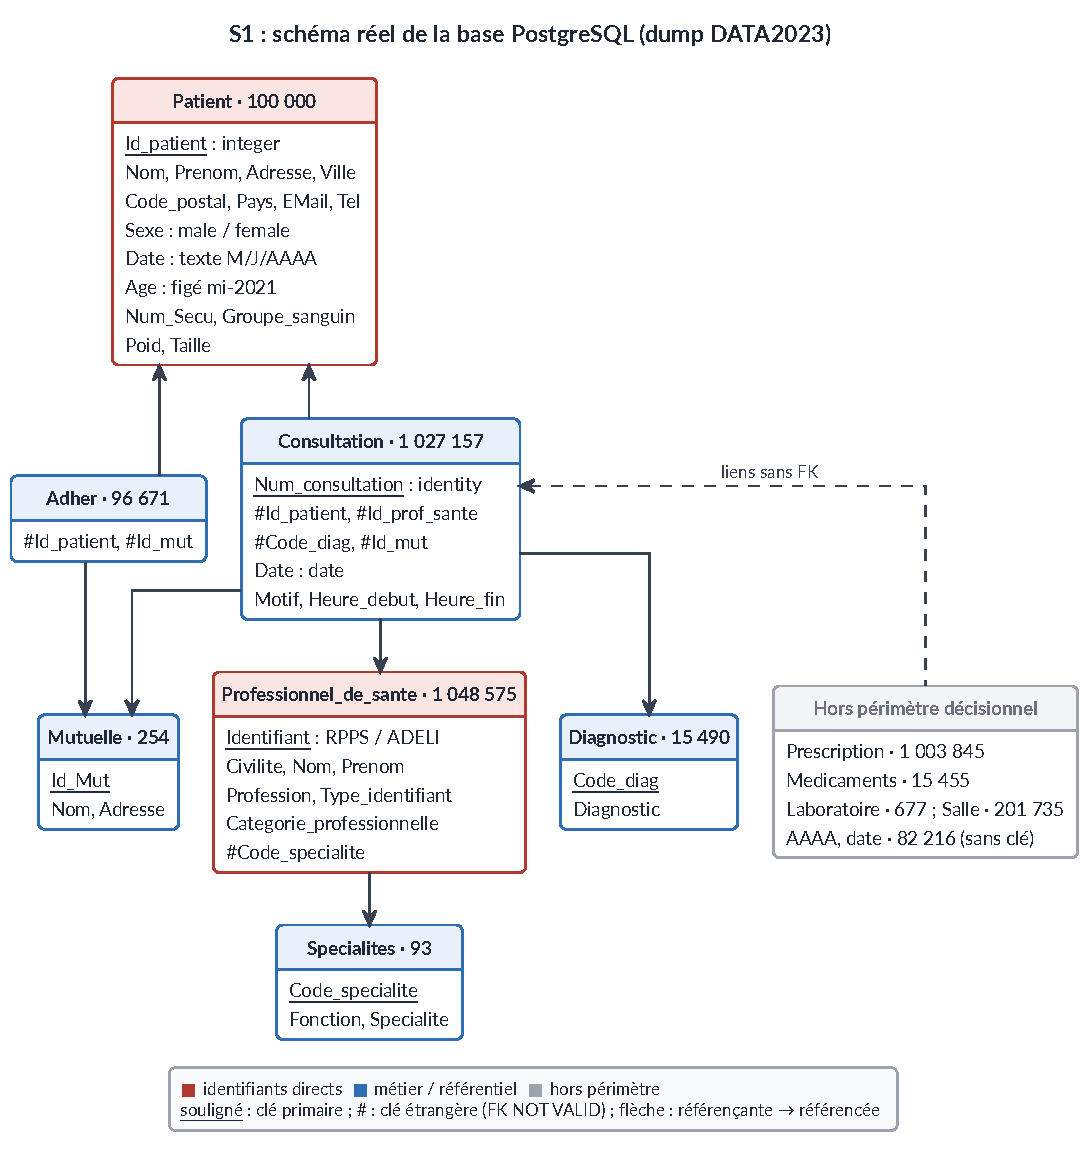
\includegraphics[width=0.8\linewidth]{figures/03_schema_source.pdf}
\caption{Schéma réel de la base S1 (MLD source, clés seulement)}\label{fig:src-db}
\end{figure}

\begin{table}[!htbp]\small
\caption{Constats de profilage et prise en charge}\label{tab:constats}
\begin{tabularx}{\linewidth}{@{}L{2.5cm}YL{2.5cm}@{}}
\toprule\entete\textbf{Source} & \textbf{Constat} & \textbf{Traitement}\\\midrule
S1 \code{Consultation} & 06/2015 à 03/2023, 0 orphelin ; \textbf{aucune colonne établissement} & RG-C04, R-01 \\
S1 \code{Patient} & Naissance en texte \code{M/J/AAAA} ; \code{Age} figé vers le 17/06/2021 ; 24\,145 consultations (2,35\,\%) avant la naissance & RG-P02, RG-C06, RQ-09 \\
S1 \code{Professionnel} & \textbf{1\,048\,575 lignes, limite d'Excel} ; 36\,170 ADELI sans zéro initial, 2 au format scientifique (\code{9,00E+34}) & RG-R01, RQ-03, RQ-14, R-02 \\
S1 \code{Mutuelle} & 44\,155 consultations (4,3\,\%) hors adhésion \code{Adher} & RQ-12 \\
S1-bis séjours & Ni sortie, ni diagnostic associé ; 2\,479 FINESS distincts & RG-H03, \Hyp{H-04} \\
S2 & \code{code\_commune} vide à 30,4\,\% (\code{cedex} renseigné) ; CP1252 ; double encodage UTF-8 des activités & RG-E03, RG-T01 \\
S3 & Séparateur, format, encodage, noms de colonnes et décimales changent par millésime ; modalités DI, NR, NV ; « recueil 2016 = données 2015 » & RG-S01 à S04, RQ-02 \\
S4 & Dates partielles ; fichiers par date d'enregistrement ; COG de l'époque ; noms sans usage & RG-D01 à D05 \\
\bottomrule
\end{tabularx}
\end{table}
Toute anomalie a une règle : de transformation (RG, ch.~\ref{chap:etl}) si une correction déterministe existe, de qualité (RQ) sinon. S3 publie des \emph{résultats agrégés par établissement} (score e-Satis ajusté, au moins 30 questionnaires \cite{has_esatis}), d'où un fait au format long piloté par une table de correspondance par millésime.

\textbf{Clés de rapprochement.}\label{tab:cles} Patient : \code{Id\_patient} (patients, consultations, séjours) $\rightarrow$ HMAC commun \code{patient\_pseudo} (RG-P01). Professionnel : S1 \code{Id\_prof\_sante} et S2 \code{identifiant}, ADELI sur 9 chiffres, RPPS sur 11 (RG-R01). Organisation : séjours, S2 \code{identifiant\_organisation}, S3 \code{finess\_geo} $\rightarrow$ \code{F} + FINESS (RG-S02). Diagnostic : \code{Code\_diag}, \code{Code\_diagnostic}, CIM-10, 0 orphelin. Géographie : S2 \code{code\_commune} ou \code{cedex}, S4 \code{code\_lieu\_deces}, S1 \code{Code\_postal} $\rightarrow$ COG courant (RG-E03, RG-D04, RG-P05).

\section{Indicateurs}\label{sec:indicateurs}
Le sujet parle de « taux » sans dénominateur : chaque indicateur reçoit une définition formelle et ses profils (D\textsubscript{G} direction du groupe, D\textsubscript{E} direction d'établissement, P praticiens, A analystes et DIM). $C$, $S$ : consultations, séjours ; $P(\cdot)$ : patients distincts ; $FA(Y)$ : file active de l'année $Y$.
\begin{table}[!htbp]\small
\caption{Définitions des indicateurs}\label{tab:indicateurs}
\begin{tabularx}{\linewidth}{@{}L{1.25cm}L{3.0cm}YL{1.35cm}@{}}
\toprule\entete\textbf{Id} & \textbf{Besoin} & \textbf{Définition (fait)} & \textbf{Profils}\\\midrule
IND-01 & Consultations dans l'établissement X & $|C(e{=}X,Y)|/|C(e\neq{-4},Y)|$, avec le taux de résolution (\code{fait\_consultation}) & D\textsubscript{G}, D\textsubscript{E}, A \\
IND-02 & Consultations pour un diagnostic X & $|C(d \in X,Y)|/|C(Y)|$ ; X = code, catégorie ou chapitre & D\textsubscript{E}, P, A \\
IND-03 & Taux global d'hospitalisation & $|P(S(Y))|/|FA(Y)|$ & D\textsubscript{G}, D\textsubscript{E}, A \\
IND-04 & Hospitalisations par diagnostic & $|S(d \in X,Y)|/|S(Y)|$ & D\textsubscript{E}, P, A \\
IND-05 & Hospitalisation par sexe et âge & IND-03 par sexe ou tranche, âge au premier contact de $Y$ & D\textsubscript{G}, P, A \\
IND-06 & Consultations par professionnel & $|C(p,Y)|/|C(Y)|$, agrégé par spécialité pour la direction & D\textsubscript{E}, P, A \\
IND-07 & Décès par région en 2019 & $\sum$ \code{nb\_deces} par région du lieu de décès au COG courant (\code{fait\_deces}) & D\textsubscript{G}, A \\
IND-08 & Satisfaction par région en 2020 & Score e-Satis 48h ajusté pondéré par l'effectif, données de 2020 (\Hyp{H-08}, \code{fait\_indicateur\_qualite}) & D\textsubscript{G}, D\textsubscript{E}, A \\
\bottomrule
\end{tabularx}
\end{table}
Limites : IND-07 est un nombre, faute de population de référence ; IND-03 à IND-05 ne valent que sur la période commune aux consultations et aux séjours (2015 à 2021).
